\documentclass[a4paper]{article}
\usepackage[14pt]{extsizes} 
\usepackage[T2A]{fontenc}
\usepackage[utf8]{inputenc}
\usepackage{natbib}
\usepackage{graphicx}
\usepackage{amsmath}
\usepackage[english, russian]{babel}
\usepackage{amsmath,amsfonts,amssymb,amsthm,mathtools,mathrsfs}
\usepackage{icomma}
\usepackage{fullpage}
\usepackage{ulem}
\usepackage{eufrak}
\usepackage{setspace}
\usepackage{listings}
\usepackage{indentfirst}
\usepackage[left=2cm,right=1.5cm,top=2cm,bottom=2cm]{geometry}
\usepackage{xcolor}
\usepackage{float}
\usepackage{csquotes}

\setlength{\parindent}{5ex}
\setlength{\parskip}{1em}
\renewcommand{\baselinestretch}{1}

\graphicspath{{images/}}

\definecolor{buzzlightyear}{HTML}{8757A5}
\definecolor{grass}{HTML}{738D06}
\definecolor{literal}{HTML}{F18A2B}
\definecolor{commentcolor}{HTML}{8E908B}

\lstdefinestyle{habrstyle}{
    backgroundcolor=\color{white},   
    commentstyle=\color{commentcolor},
    keywordstyle=\bfseries\color{buzzlightyear},
    numberstyle=\tiny\color{commentcolor},
    stringstyle=\color{grass},
    basicstyle=\ttfamily\footnotesize,
    breakatwhitespace=false,         
    breaklines=true,                 
    captionpos=b,                    
    keepspaces=true,                 
    numbers=left,                    
    numbersep=5pt,                  
    showspaces=false,                
    showstringspaces=false,
    showtabs=false,                  
    tabsize=4
}

\lstset{style=habrstyle}

\begin{document}
    % НАЧАЛО ТИТУЛЬНОГО ЛИСТА
    \begin{center}
        \begin{center}
        \hfill \break
        \normalsize{Санкт-Петербургский государственный политехнический}\\
        \normalsize{университет Петра Великого}\\
        \hfill \break
        \normalsize{\textbf{Высшая школа интеллектуальных систем и}}\\ 
        \normalsize{\textbf{суперкомпьютерных технологий}}\\ 
        \hfill \break
        \hfill \break
        \hfill \break
        \normalsize{Лабораторная работа №2}\\
        \hfill \break
        \hfill \break
        \normalsize{\LARGE Гармоники}\\
        \end{center}
        \hfill \break
        \hfill \break
        \hfill \break
        \hfill \break
        \hfill \break
        \hfill \break
        \hfill \break
        \hfill \break
        \hfill \break
        \hfill \break
       \begin{flushright}
            \normalsize{Выполнил студент 3-го курса}\\
            \normalsize{группа 3530901/80201}\\
            \normalsize{Матвеец Андрей Вадимович}\\
            \hfill \break
            \normalsize{Преподаватель:}\\
            \normalsize{Богач Наталья Владимировна}\\
        \end{flushright}
        \hfill \break
        \hfill \break
        \hfill \break
        \hfill \break
        \begin{center} Санкт-Петербург\end{center}
        \begin{center}2021\end{center} 
        \thispagestyle{empty}
    \end{center}
    % КОНЕЦ ТИТУЛЬНОГО ЛИСТА
    
    % ОГЛАВЛЕНИЕ
    \newpage
        \tableofcontents
    
    % СПИСОК ИЛЛЮСТРАЦИЙ
    \newpage
         \listoffigures
    
    % СПИСОК ЛИСТИНГОВ     
    \newpage
         \lstlistoflistings   
     
    \newpage
        \section{Часть №1: Запуск примеров из \texttt{chap02.ipynb}}
            В первом пункте лабораторной работы нам необходимо выполнить программы из файла \texttt{chap02.ipynb}. 
            
             \begin{figure}[h]
                \centering
                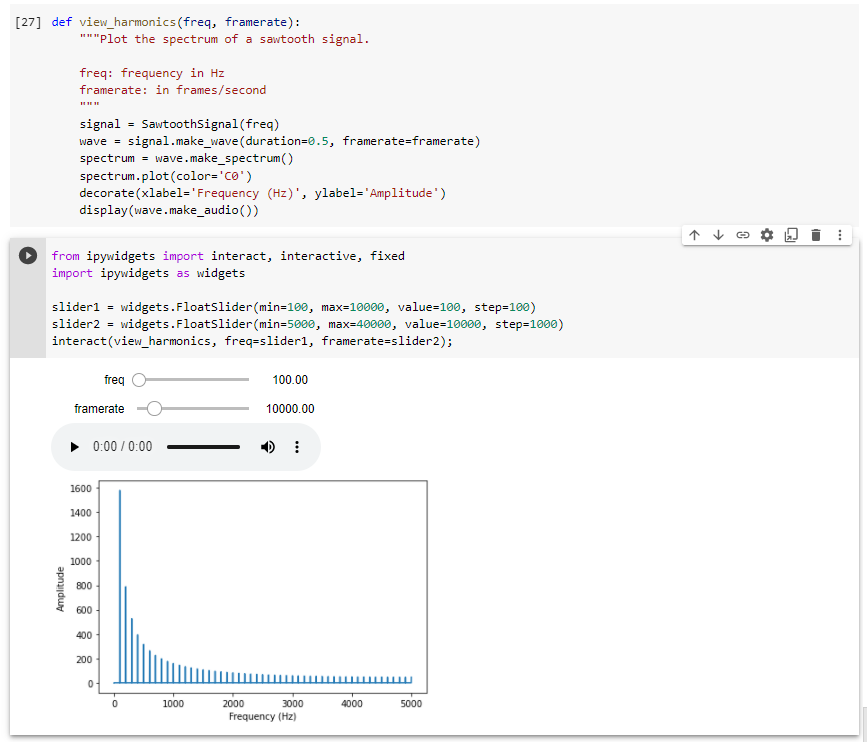
\includegraphics[width=\textwidth]{ex_1_all_work.png}
                \caption{Проверка работоспособности}
                \label{fig:check_it_works}
            \end{figure}
            
            В результате выполнения мы увидели, что все запускается как ожидалось, никаких проблем с запуском не появилось и можно переходить к выполнению следующего пункта.
    
    \newpage
        \section{Часть №2: Создание \texttt{SawtoothSignal}}
            Во втором пункте лабораторной работы нам необходимо создать класс \texttt{SawtoothSignal}, расширяющий \texttt{signal} и предоставляющий \texttt{evaluate} для оценки пилообразного сигнала. Необходимо так же вычислить спектр пилообразного сигнала.
            
            Начнем с подключения необходимых нам библиотек и создания класса \\
            \texttt{SawtoothSignal}
            
\begin{lstlisting}[language=Python, caption= Создание класса \texttt{SawtoothSignal}]
    from thinkdsp import decorate, Sinusoid, normalize, unbias, TriangleSignal, SquareSignal, SinSignal, CosSignal, ParabolicSignal

    import numpy as np

    class SawtoothSignal(Sinusoid):
        def evaluate(self, ts):
            cycles = self.freq * ts + self.offset / np.pi / 2
            
            frac, _ = np.modf(cycles)
            ys = normalize(unbias(frac), self.amp)
            return ys
\end{lstlisting}    
            
            Теперь проверим, что написанный класс \texttt{SawtoothSignal} работает корректно, для этого обратимся к данному классу и преобразуем все в волну, после чего выведем на экран.

\begin{lstlisting}[language=Python, caption= Тестирование класса \texttt{SawtoothSignal}]
    test_saw = SawtoothSignal()
    test_wave = test_saw.make_wave(test_saw.period * 5, framerate=40000)
    test_wave.plot()
    decorate(xlabel='Time (s)')
\end{lstlisting}               
            
            \begin{figure}[H]
                \centering
                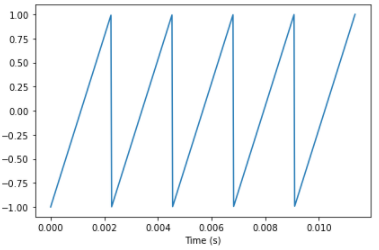
\includegraphics[width=\textwidth]{ex_2_test_class.png}
                \caption{Проверка написанного класса \texttt{SawtoothSignal}}
                \label{fig:test_class}
            \end{figure}
            
            После этого получим аудио дорожку, обращаясь к классу:
            
            \begin{figure}[H]
                \centering
                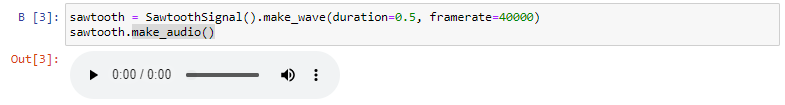
\includegraphics[width=\textwidth]{ex_2_class_audio.png}
                \caption{Получение аудиодорожки из написанного класса \texttt{SawtoothSignal}}
                \label{fig:class_audio}
            \end{figure}
            
            Теперь построим спектр:
            
\begin{lstlisting}[language=Python, caption= Построение спектра]
    sawtooth.make_spectrum().plot()
    decorate(xlabel='Frequency (Hz)')
\end{lstlisting}               
            
            \begin{figure}[H]
                \centering
                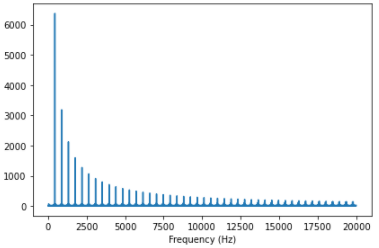
\includegraphics[width=\textwidth]{ex_2_class_spectr_1.png}
                \caption{Построение спектра}
                \label{fig:class_spectr_1}
            \end{figure}
            
            Также сравним наш пилообразный сигнал сначала с прямоугольной волной:
            
\begin{lstlisting}[language=Python, caption= Построение прямоугольной волны]
    sawtooth.make_spectrum().plot(color='gray')
    square = SquareSignal(amp=0.5).make_wave(duration=0.5, framerate=40000)
    square.make_spectrum().plot()
    decorate(xlabel='Frequency (Hz)')
\end{lstlisting}               
            
            \begin{figure}[H]
                \centering
                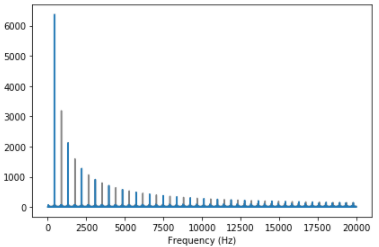
\includegraphics[width=\textwidth]{ex_2_compare_square.png}
                \caption{Построение прямоугольной волны}
                \label{fig:compare_square}
            \end{figure}
            
            Также для сравнения получим аудио из прямоугольного сигнала:
            
            \begin{figure}[H]
                \centering
                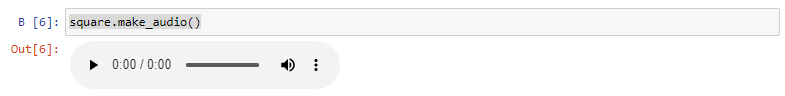
\includegraphics[width=\textwidth]{ex_2_compare_square_audio.png}
                \caption{Получение аудио из прямоугольного сигнала}
                \label{fig:compare_square_audio}
            \end{figure}
            
            Теперь сравним наш пилообразный сигнал с треугольным сигналом:
            
\begin{lstlisting}[language=Python, caption= Построение треугольной волны]
    sawtooth.make_spectrum().plot(color='gray')
    triangle = TriangleSignal(amp=0.79).make_wave(duration=0.5, framerate=40000)
    triangle.make_spectrum().plot()
    decorate(xlabel='Frequency (Hz)')
\end{lstlisting}               
            
            \begin{figure}[H]
                \centering
                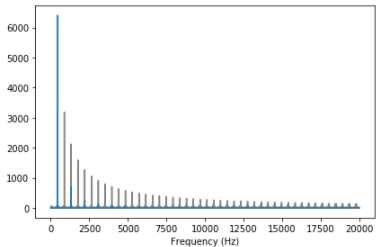
\includegraphics[width=\textwidth]{ex_2_compare_triangle.png}
                \caption{Построение треугольгой волны}
                \label{fig:compare_triangle}
            \end{figure}
            
            Также для сравнения получим аудио из треугольного сигнала:
            
            \begin{figure}[H]
                \centering
                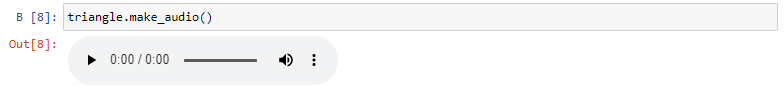
\includegraphics[width=\textwidth]{ex_2_compare_triangle_audio.png}
                \caption{Получение аудио из треугольного сигнала}
                \label{fig:compare_triangle_audio}
            \end{figure}
            
            В результате выполнения данного пункта можно сделать вывод о том, что в нашем пилообразном сигнале амплитуды частот уменьшаются пропорционально самой частоте, а не ее квадрату. Кроме того при сравнении аудио полученных прямоугольных и треугольных сигналов можно сказать, что квадратный звучит намного реже пилообразного, в то время как треугольный звучит тише.
            
    \newpage
        \section{Часть №3: Квадратный сигнал}
            В третьей части лабораторной работы нам необходимо создать треугольный сигнал \texttt{1100 Hz} и вычислить \texttt{wave} с выборками 10000 кадров в секунду. Также необходимо построить спектр и убедиться, что большинство гармоник "завернуты" из-за биений.
            
            Для начала создадим прямоугольный сигнал:
            
\begin{lstlisting}[language=Python, caption= Построение прямоугольного сигнала]
    signal = SquareSignal(1100)
    wave = signal.make_wave(duration=0.5, framerate=10000)
\end{lstlisting}       
            
            После этого построим спектр для этого сигнала:
            
\begin{lstlisting}[language=Python, caption= Построение спектра]
    spectr = wave.make_spectrum()
    spectr.plot()
    decorate(xlabel='Frequency (Hz)')
\end{lstlisting}               
            
            \begin{figure}[H]
                \centering
                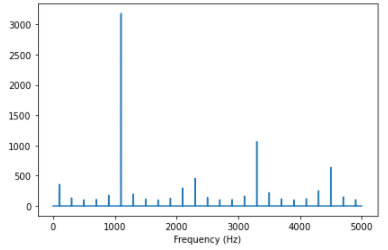
\includegraphics[width=\textwidth]{ex_3_square.png}
                \caption{Построеный спектр}
                \label{fig:ex_3_square}
            \end{figure}
            
            Также создадим из данного сигнала аудиодорожку:
            
            \begin{figure}[H]
                \centering
                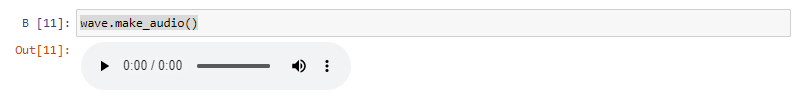
\includegraphics[width=\textwidth]{ex_3_square_audio.png}
                \caption{Аудио из прямоугольного сигала}
                \label{fig:ex_3_square_audio}
            \end{figure}
            
            Для сравнения, чтобы понять, что мы можем услышать «\texttt{aliased}-частоты» создадим еще один сигнал, в нашем случаем синусоидальный
            
\begin{lstlisting}[language=Python, caption= Построение синусоидального сигнала]
    signal2 = SinSignal(1000)
    wave2 = signal2.make_wave(duration=0.5, framerate=5000)
\end{lstlisting}    
            
            Теперь так же создадим для него спектр:
            
\begin{lstlisting}[language=Python, caption= Построение спектра]
    spectr2 = wave2.make_spectrum()
    spectr2.plot()
    decorate(xlabel='Frequency (Hz)')
\end{lstlisting}               
            
            \begin{figure}[H]
                \centering
                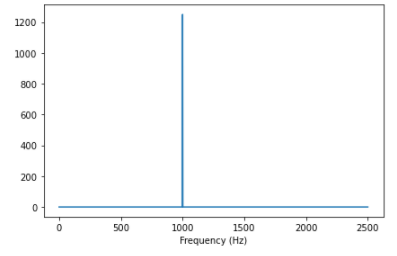
\includegraphics[width=\textwidth]{ex_3_sin.png}
                \caption{Построеный спектр}
                \label{fig:ex_3_sin}
            \end{figure}
            
            Также создадим из данного сигнала аудиодорожку:
            
            \begin{figure}[H]
                \centering
                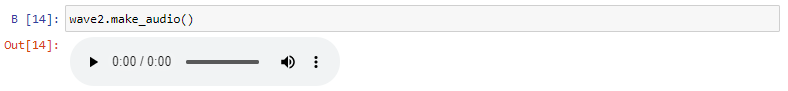
\includegraphics[width=\textwidth]{ex_3_sin_audio.png}
                \caption{Аудио из синусоидального сигала}
                \label{fig:ex_3_sin_audio}
            \end{figure}
            
            В результате выполнения данного пункта мы можем сравнить эти 2 сигнала. На слух они очень сильно отличаются друг от друга, первый сигнал очень сильно режет слух и присутствует некая пульсация. Так как эти два аудио слышатся по разному, значит мы можем расслышать «\texttt{aliased}-частоты»
            
    \newpage
        \section{Часть №4: Нулевая частота}
            В четвертой части лабораторной работы нам необходимо взять объект \texttt{spectrum} и распечатать несколько первых значений \texttt{spectrum.hs}. Необходимо также убедиться, что они начинаются с нуля, т.е. \texttt{spectrum.hs[0]} - амплитуда компоненты с частотой 0.
            
                \begin{enumerate}
                    \item Создать треугольный сигнал с частотой \texttt{440 Hz} и \texttt{wave} длительностью 0.01 с. после чего распечатать сигнал.
                    \item Создать объект \texttt{spectrum} и распечатать \texttt{spectrum.hs[0]}. Определить какая амплитуда и фаза у компонента.
                    \item Установить \texttt{spectrum.hs[0]} = 100 и определить как данная операция влияет на сигнал.
                \end{enumerate}
            
            Для начала создадим треугольный сигнал согласно заданию:
            
\begin{lstlisting}[language=Python, caption= Построение треугольного сигнала]
    triangle = TriangleSignal(440)
    wave = triangle.make_wave(duration=0.01)
    wave.plot()
    decorate(xlabel='Time (s)')
\end{lstlisting}               
            
            \begin{figure}[H]
                \centering
                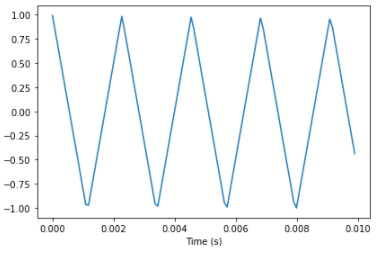
\includegraphics[width=\textwidth]{ex_4_triangle_signal.png}
                \caption{Построеный треугольный сигнал}
                \label{fig:ex_4_triangle_signal}
            \end{figure}
            
            После этого создадим спектр для данного сигнала:
            
\begin{lstlisting}[language=Python, caption= Спектр треугольного сигнала]
    spectrum = wave.make_spectrum()
    spectrum.plot()
    decorate(xlabel='Frequency (Hz)')
\end{lstlisting}               
            
            \begin{figure}[H]
                \centering
                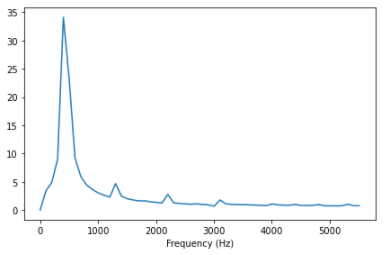
\includegraphics[width=\textwidth]{ex_4_triangle_signal_spectr.png}
                \caption{Спектр треугольного сигнала}
                \label{fig:ex_4_triangle_signal_spectr}
            \end{figure}
            
            Теперь посмотрим на \texttt{spectrum.hs[0]}
            
            \begin{figure}[H]
                \centering
                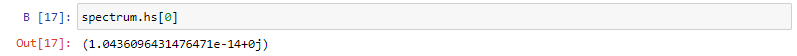
\includegraphics[width=\textwidth]{ex_4_spectrum_hs.png}
                \caption{\texttt{spectrum.hs[0]}}
                \label{fig:ex_4_spectrum_hs}
            \end{figure}
            
            Как можно увидеть, \texttt{spectrum.hs[0]} равен \texttt{1.0436096431476471e-14+0j}. "Длина" данного числа описывает амплитуту нулевой компоненты разложения, а угол с \texttt{Re} описывает частоту.
            
            Наконец, установим \texttt{spectrum.hs[0]} = 100 и выведем полученный сигнал выведем на экран
            
\begin{lstlisting}[language=Python, caption= \texttt{spectrum.hs[0]} = 100]
    spectrum.hs[0] = 100
    wave.plot(color='gray')
    spectrum.make_wave().plot()
    decorate(xlabel='Time (s)')
\end{lstlisting}               
            
            \begin{figure}[H]
                \centering
                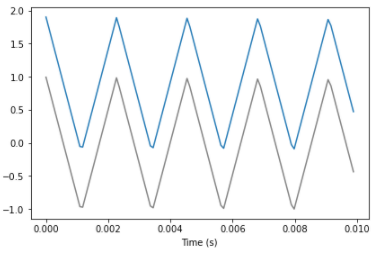
\includegraphics[width=\textwidth]{ex_4_triangle_signal_compare.png}
                \caption{\texttt{spectrum.hs[0]} = 100}
                \label{fig:ex_4_triangle_signal_compare}
            \end{figure}
            
            Как можно видеть в результате выполнения данного пункта, нет совершенно никакой разницы между полученными сигналами.
    
    \newpage
        \section{Часть №5: Деление амплитуды на частоту}
            В пятом пункте лабораторной работы нам необходимо создать функцию, приннимающую \texttt{spectrum} как параметр и изменяющую его делением каждого элемента \texttt{hs} на соответствующую частоту из \texttt{fs}.
            Необходимо также проверить данную функцию на прямоугольном, треугольном или пилообразном сигнале.
            
                \begin{enumerate}
                    \item Вычислить \texttt{spectrum} и распечатать его
                    \item Изменить \texttt{spectrum}, использую нашу функцию, и распечатать его.
                    \item Использовать \texttt{spectrum.make-wave}, чтобы сделать \texttt{wave} из измененного \texttt{spectrum} и прослушать его. Как изменился сигнал?
                \end{enumerate}
                
            Для начала напишем нашу функцию \texttt{filter-spectrum}:
            
\begin{lstlisting}[language=Python, caption= filter-spectrum]
    def filter_spectrum(spectrum):
    spectrum.hs[1:] /= spectrum.fs[1:]
    spectrum.hs[0] = 0
\end{lstlisting}  
           
           После этого создадим прямоугольный сигнал и сразу переведем его в аудио

            \begin{figure}[H]
                \centering
                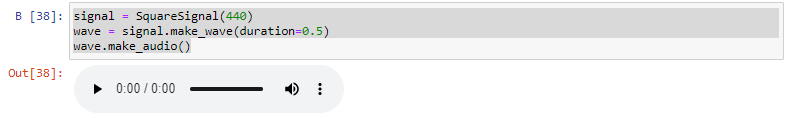
\includegraphics[width=\textwidth]{ex_5_square_signal.png}
                \caption{Прямоугольный сигнал}
                \label{fig:ex_5_square_signal}
            \end{figure}
            
            После этого сразу выведем на экран спектр исходного сигнала, после чего отдадим его на вход нашей функции. После этого так же выведем полученный спектр на экран:
            
\begin{lstlisting}[language=Python, caption= Работа с сигналами]
    spectrum = wave.make_spectrum()
    spectrum.plot(high=10000, color='gray')
    filter_spectrum(spectrum)
    spectrum.scale(440)
    spectrum.plot(high=10000)
    decorate(xlabel='Frequency (Hz)')
\end{lstlisting}               
            
            \begin{figure}[H]
                \centering
                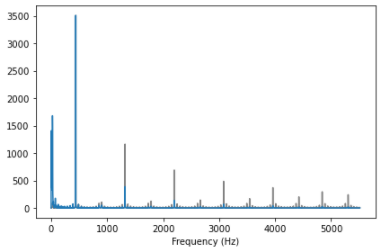
\includegraphics[width=\textwidth]{ex_5_spectr_compare.png}
                \caption{Вывод спектров на экран}
                \label{fig:ex_5_spectr_compare}
            \end{figure}
           
           Теперь так же переведем полученный сигнал в аудио:
           
            \begin{figure}[H]
                \centering
                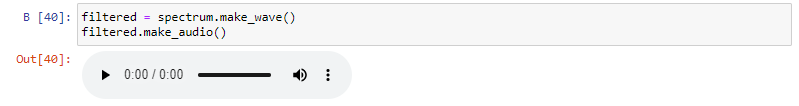
\includegraphics[width=\textwidth]{ex_5_result_signal_audio.png}
                \caption{Полученный сигнал в аудио}
                \label{fig:ex_5_result_signal_audio}
            \end{figure}
           
           В результате выполнения данного пункта можно сказать о том, что полученный сигнал звучит тише, чем изначальный сигнал. Он уже не режет уши, как оригинальный сигнал.
           
    \newpage
        \section{Часть №6: Нахождение сигнала}   
            В шестой части второй лабораторной работы нам необходимо определить, можно ли найти сигнал, состоящий из четныз и нечетных гармоник, спадающих пропорционально 1/$f^2$ ?
            
            Сам текст программы:
            У треугольных и прямоугольных сигналов есть только нечетные гармоники; в пилообразном сигнале есть и четные, и нечетные гармоники. Гармоники прямоугольных и пилообразных сигналов уменьшаются пропорционально 1/$f^2$ гармоники треугольных сигналов — пропорционально 1/$f^2$. Можно ли найти сигнал, состоящий из четных и нечетных гармоник, спадающих пропорционально 1/$f^2$?
            
            Для начала  создадим пилообразный сигнал и представим его в виде аудио
            
             \begin{figure}[H]
                \centering
                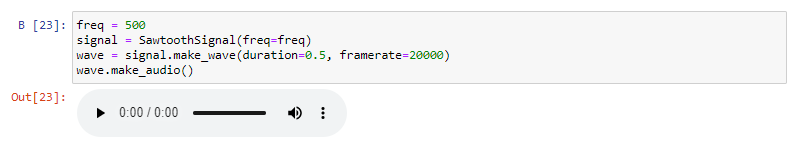
\includegraphics[width=\textwidth]{ex_6_sawtooth_signal_audio.png}
                \caption{Пилообразный сигнал в аудио}
                \label{fig:ex_6_sawtooth_signal_audio}
            \end{figure}
            
            После этого выведем его на экран:
            
\begin{lstlisting}[language=Python, caption= Вывод пилообразного сигнала на экран]
    wave_plot = signal.make_wave(duration=signal.period*10, framerate=20000)
    wave_plot.plot()
    decorate(xlabel='Time (s)')
\end{lstlisting}               
            
            \begin{figure}[H]
                \centering
                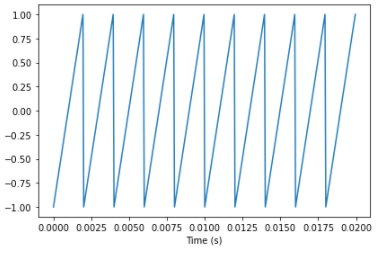
\includegraphics[width=\textwidth]{ex_6_sawtooth_signal_plot.png}
                \caption{Вывод пилообразного сигнала на экран}
                \label{fig:ex_6_sawtooth_signal_plot}
            \end{figure}
            
            Теперь представим его в виде спектра и так же выведем на экран:
            
\begin{lstlisting}[language=Python, caption= Вывод спектра на экран]
    spectrum = wave.make_spectrum()
    spectrum.plot()
    decorate(xlabel='Frequency (Hz)')
\end{lstlisting}               
            
            \begin{figure}[H]
                \centering
                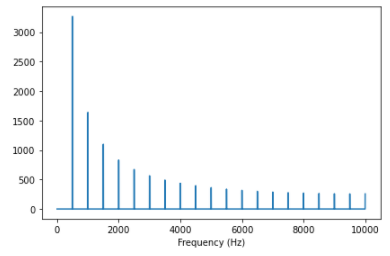
\includegraphics[width=\textwidth]{ex_6_sawtooth_spectrum.png}
                \caption{Вывод спектра на экран}
                \label{fig:ex_6_sawtooth_spectrum}
            \end{figure}
            
            После всего этого нам необходимо вызвать функцию, написанную в прошлом задании, и применить к нашему текущему спектру. Сразу после этого выведем полученный спектр на экран:
            
\begin{lstlisting}[language=Python, caption= Вызов функции и вывод нового спектра на экран]
    spectrum.plot(color='gray')
    filter_spectrum(spectrum)
    spectrum.scale(freq)
    spectrum.plot()
    decorate(xlabel='Frequency (Hz)')
\end{lstlisting}               
            
            \begin{figure}[H]
                \centering
                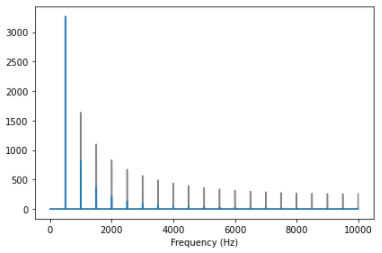
\includegraphics[width=\textwidth]{ex_6_sawtooth_spectrum_fun.png}
                \caption{Вывод нового спектра на экран}
                \label{fig:ex_6_sawtooth_spectrum_fun}
            \end{figure}
            
            Наконец переведем полученный сигнал в аудио:
            
            \begin{figure}[H]
                \centering
                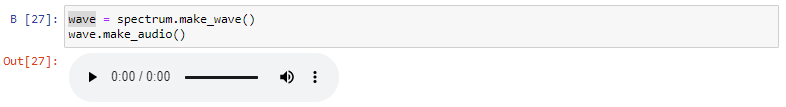
\includegraphics[width=\textwidth]{ex_6_sawtooth_spectrum_fun_audio.png}
                \caption{Перевод полученного сигнала в аудио}
                \label{fig:ex_6_sawtooth_spectrum_fun_audio}
            \end{figure}
            
            Сразу после этого преобразуем наш спектр в сегменты и выведем так же на экран:
            
\begin{lstlisting}[language=Python, caption= Преобразование спектра в сегменты и вывод на экран]
    wave.segment(duration=0.03).plot()
    decorate(xlabel='Time (s)')
\end{lstlisting}               
            
            \begin{figure}[H]
                \centering
                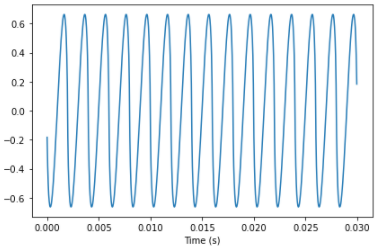
\includegraphics[width=\textwidth]{ex_6_sawtooth_spectrum_fun_segment.png}
                \caption{Вывод нового спектра на экран}
                \label{fig:ex_6_sawtooth_spectrum_fun_segment}
            \end{figure}
            
            Также можно выполнить другой подход, а именно - сложить серию косинусоидальных сигналов с парвильными частотами и амплитудами. Код реализующий это представлен ниже:
            
\begin{lstlisting}[language=Python, caption= Другой подход]
    freqs = np.arange(500, 9500, 500)
    amps = 1 / freqs**2
    signal = sum(CosSignal(freq, amp) for freq, amp in zip(freqs, amps))
    signal
\end{lstlisting}   

        Отобразим спектр полученного сигнала:
        
\begin{lstlisting}[language=Python, caption= Отображение спектра нового сигнала]
    spectrum = wave.make_spectrum()
    spectrum.plot()
    decorate(xlabel='Frequency (Hz)')
\end{lstlisting}               
            
            \begin{figure}[H]
                \centering
                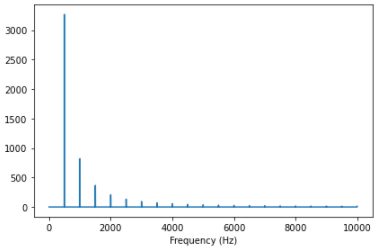
\includegraphics[width=\textwidth]{ex_6_sawtooth_spectrum_result.png}
                \caption{Вывод нового спектра на экран}
                \label{fig:ex_6_sawtooth_spectrum_result}
            \end{figure}
            
            Преобразуем новый сигнал в файл:
            
            \begin{figure}[H]
                \centering
                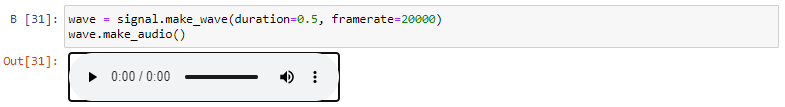
\includegraphics[width=\textwidth]{ex_6_sawtooth_spectrum_result_audio.png}
                \caption{Преобразование нового спектра в аудио}
                \label{fig:ex_6_sawtooth_spectrum_result_audio}
            \end{figure}
            
            Наконец, преобразуем наш новый сигнал в сегменты и так же отобразим их на экране:
            
\begin{lstlisting}[language=Python, caption= Отображение сегментов нового сигнала]
    wave.segment(duration=0.03).plot()
    decorate(xlabel='Time (s)')
\end{lstlisting}               
            
            \begin{figure}[H]
                \centering
                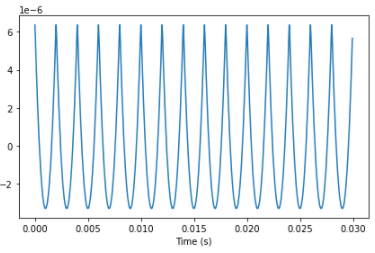
\includegraphics[width=\textwidth]{ex_6_sawtooth_segment_result.png}
                \caption{Отображение сегментов нового сигнала}
                \label{fig:ex_6_sawtooth_segment_result}
            \end{figure}
            
            Как можно увидеть, полученный нами результат похож на параболы, что является правдой, от части. Этот же результат можно добиться, использовав астроенную в \texttt{thinkdsp} библиотеку \texttt{ParabolicSignal}, вычисляющую параболические формы волны.
            
            Создадим новый сигнал на основе \texttt{ParabolicSignal} и переведем его сразу в аудио:
            
            \begin{figure}[H]
                \centering
                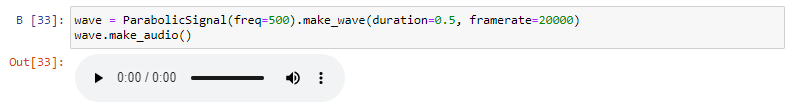
\includegraphics[width=\textwidth]{ex_6_parabolicSignal_audio.png}
                \caption{Создание сигнала через \texttt{ParabolicSignal}}
                \label{fig:ex_6_parabolicSignal_audio}
            \end{figure}
            
            После этого создадим сегменты из нового сигнала и посмотрим на них:
            
\begin{lstlisting}[language=Python, caption= Отображение сегментов нового сигнала \texttt{ParabolicSignal}]
    wave.segment(duration=0.03).plot()
    decorate(xlabel='Time (s)')
\end{lstlisting}               
            
            \begin{figure}[H]
                \centering
                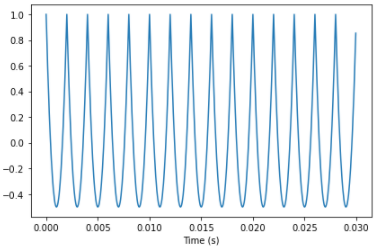
\includegraphics[width=\textwidth]{ex_6_parabolicSignal_segment.png}
                \caption{Отображение сегментов нового сигнала \texttt{ParabolicSignal}}
                \label{fig:ex_6_parabolicSignal_segment}
            \end{figure}
            
            В результате выполнения данного пункта можно сказать, что полученные аудиодорожки результата и из \texttt{ParabolicSignal} абсолютно идентичны, в результате чего можно сделать вывод, что это один и тот же сигнал.
            
    \newpage
        \section{Выводы}
            В результате выполнения данной лабораторной работы мы изучили способы работы с гармониками, их обработки, смены параметров и т.д. Кроме того был реализован и проверен класс для оценки пилообразного сигнала. Также была создана функция для изменения \texttt{spectrum} путем изменения его делением каждого элемента \texttt{hs} на соответствующую частоту из \texttt{fs}. 
\end{document}
